\section{Empirical details and full result tables}
\label{app:empirical}

This appendix collects the complete result tables underlying
Section~\ref{sec:results}. Tables are placed inline with \texttt{[h]} so that
each appears with its heading.

\subsection{Single-section model comparison}
\begin{figure}[h]
  \centering
  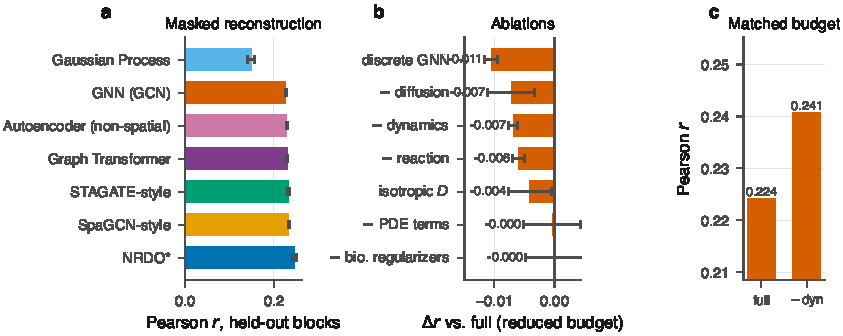
\includegraphics[width=\linewidth]{figures/fig_results_panel.pdf}
  \caption{\textbf{Locating the effect} on the primary section, where all nine
  models are run. (a) Full model comparison. (b) Ablation deltas at the reduced
  budget. (c) The two decisive controls at the benchmark budget: disabling the
  operator ($T{=}0$) costs more than the full margin over the best baseline.}
  \label{fig:results}
\end{figure}


\subsection{Numerical behavior}
\begin{figure}[h]
  \centering
  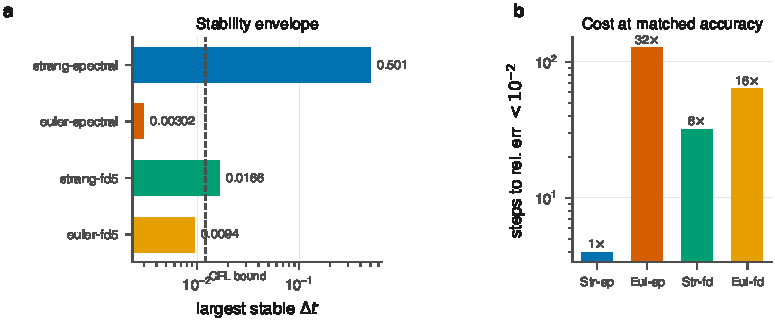
\includegraphics[width=\linewidth]{figures/fig_numerics.pdf}
  \caption{\textbf{What the exact spectral solve buys.} (a) Largest stable step
  size per scheme against the CFL bound for the explicit five-point Laplacian.
  (b) Steps required to integrate a fixed horizon to relative error $<10^{-2}$,
  relative to the exponential scheme.}
  \label{fig:numerics}
\end{figure}


\subsection{Paired statistics, numerics and biology}
\inputtable{tab_paired}
\inputtable{tab_numerics}
\inputtable{tab_biology}

\subsection{Dataset inventory}
\inputtable{tab_datasets}

\subsection{Ablation sweep}
Full sweep at the reduced budget; the two matched-budget controls are reported in
Section~\ref{sec:ablations}.
\inputtable{tab_ablations}

\subsection{Cross-tissue and cross-resolution transfer}
\inputtable{tab_transfer_tissue}
\inputtable{tab_transfer_resolution}

\subsection{Developmental forecasting}
Horizon sweep for E9.5 $\rightarrow$ E10.5. Consecutive MOSTA stages are distinct
embryos, so the comparison is at the level of the rasterized field after
isotropic normalization to a common frame.
\inputtable{tab_development}

\subsection{In-silico morphogen source}
Split-half protocol of Section~\ref{sec:results4}: the perturbation direction is
defined from a random half of each pathway and enrichment scored on the held-out
half, against a permutation null over matched gene sets.
\inputtable{tab_bead}

\subsection{Perturb-seq consistency}
An out-of-context probe: Norman et al.\ profiled non-spatial K562 cells whereas
the operator is fitted to tissue. With $n=\PSNPerturb$ testable perturbations the
comparison is underpowered and we report it as inconclusive.
\inputtable{tab_perturbseq}

\subsection{Latent fields}
\label{app:latent}
\begin{figure}[h]
  \centering
  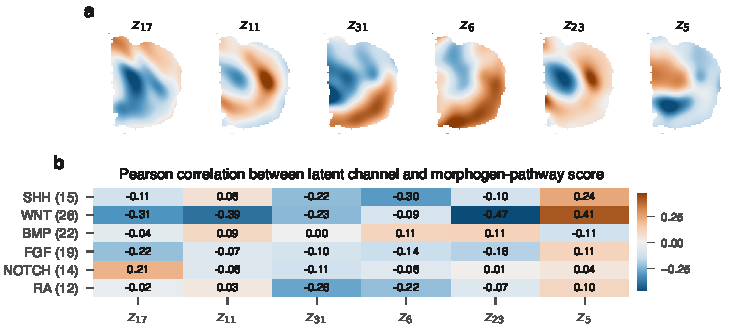
\includegraphics[width=\linewidth]{figures/fig3_latent_fields.pdf}
  \caption{Latent channels of the relaxed field (a) and their correlation with
  canonical morphogen-pathway scores (b). Section~\ref{sec:results4} shows these
  correlations do not survive a causal split-half test.}
  \label{fig:latent}
\end{figure}
